\section{State Space Analysis}
\label{sec:State_Space_Analysis}

In order to describe the utility of state space-based analysis, we consider the simplified version of a trajectory planning application requiring strict temporal behavior. The component assembly for this application is shown in Figure \ref{fig:tpa}. This application consists of two components: A \emph{Sensor} component and a \emph{Trajectory Planner} component. The Sensor component periodically publishes on a trigger topic, notifying the Trajectory Planner of the existence of new sensor data. Once the notification is received, the Trajectory Planner makes an RMI call to retrieve the data structure of sensor values. Using the updated sensor values, the Trajectory Planner calculates a new trajectory for the satellite. 

\begin{figure}[ht]
\centering
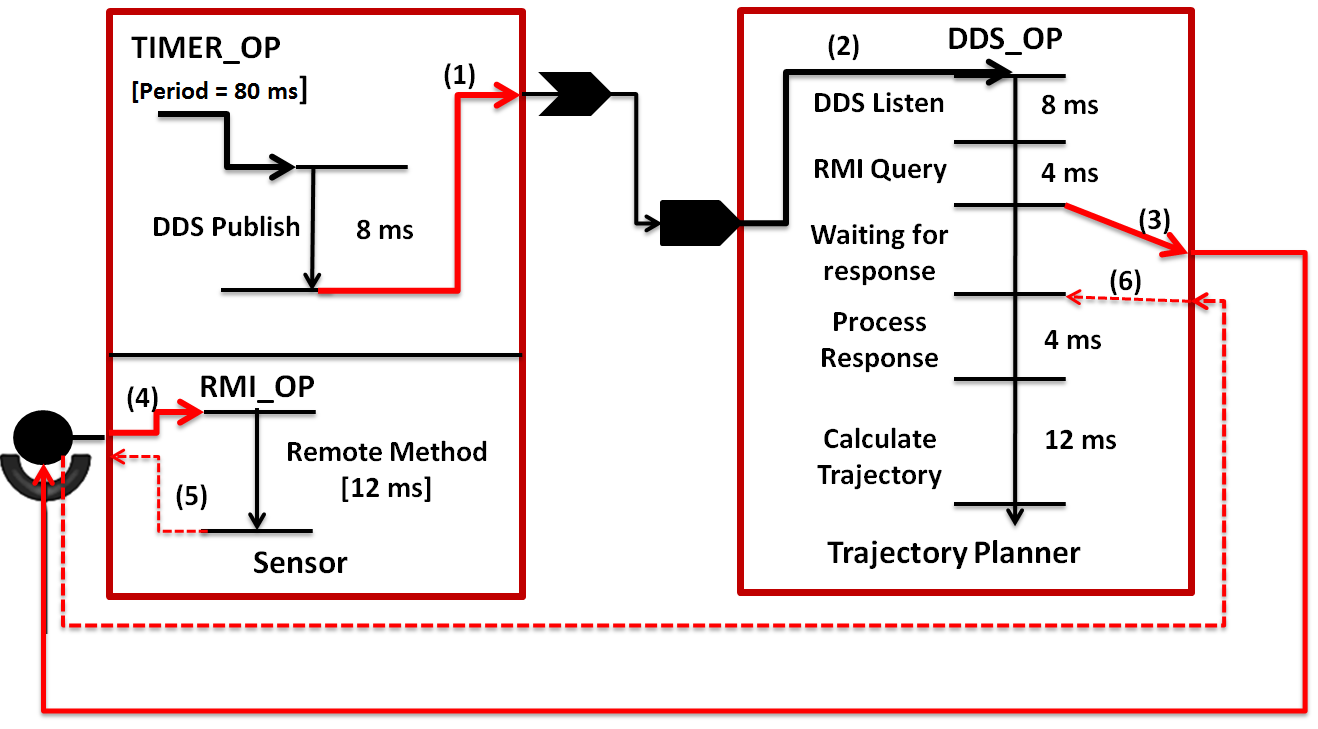
\includegraphics[width=0.5\textwidth]{tpa}
\caption{Trajectory Planning Application}
\label{fig:tpa}
\vspace{-0.2in}
\end{figure}
%\vspace{0.1in}

\begin{figure}[ht]
\centering
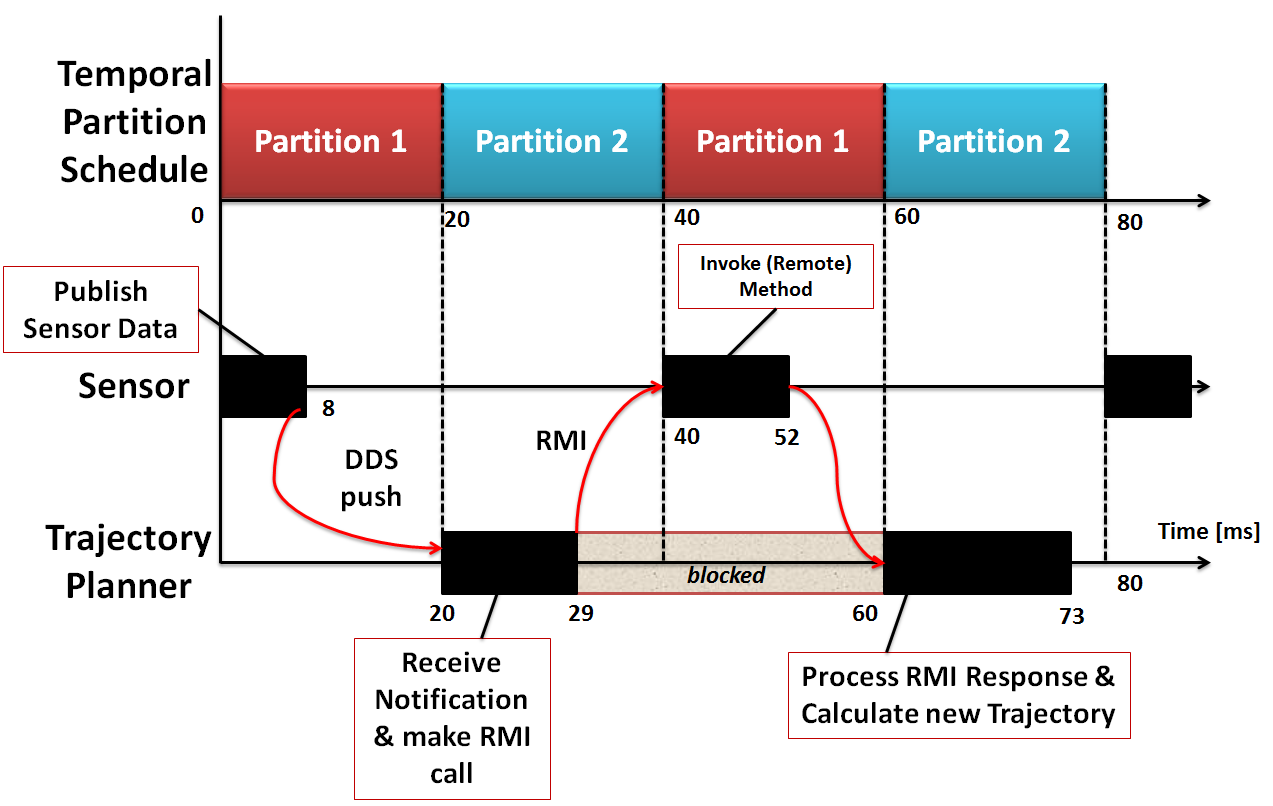
\includegraphics[width=0.5\textwidth]{tpa_td}
\caption{Timing Diagram for Trajectory Planning}
\label{fig:tpa_td}
\vspace{-0.2in}
\end{figure}
\vspace{0.1in}

Figure \ref{fig:tpa_td} shows the partition schedule and temporal behavior considered. The sensor component operates on partition 1, and the trajectory planner operates on partition 2. Both partitions have a duration of 20 ms and a period of 40 ms. The sensor component is associated with a periodic timer that fires every 80 ms. When this timer expires, the sensor component publishes on a notification topic. Accounting for network latencies, the analysis assumes that this task does not take more than 8 ms. Once the notification is sent out, the sensor component becomes passive. With DDS push semantics, this notification manifests itself as a DDS operation on the trajectory planner's message queue. When partition 2 becomes active, the trajectory planner component receives the notification is has subscribed to, after which it makes an RMI call to the sensor component to obtain the updated sensor values. After the RMI call is made, this component blocks for the remainder of the partition. When the sensor component is scheduled again, it services the RMI request and sends out the RMI response, effectively unblocking the trajectory planner. Once the new sensor data is retrieved, the trajectory planner calculates a new trajectory for the satellite node. %	For the sake of analysis, we assume the temporal behavior shown in Figure \ref{fig:tpa}.

%Using the in-built state space tool, a complete or partial state space can be generated for the modeled system. Partial state spaces are generated by specifying predicates or limiting paramters e.g. number of state space nodes. Once generated, a standard report summarizes the results. This report provides information  on: (1) Size of the state space, (2) Boundedness Properties for all the places in the model, (3) Liveness Properties for all transitions in the model, (4) Fairness Properties for transition  firings, and (5) Home Properties for home markings. It is, however, not necessary to generate this report as all of this information can be derived using the \emph{Evaluate ML} feature in CPN Tools. Here, state space queries are written as auxiliary text in the model and evaluated as standard ML code. 

%\vspace{-0.15in}
\subsection{Deadline Violation Detection}

Using the \emph{op\_st} and \emph{op\_et} fields of every component operation, the model is capable of identifying deadline violations in component operations that are either currently in progress or waiting in the component message queue. The model essentially takes a snapshot of such cases and records the time stamps. For instance: In Figure \ref{fig:tpa_td}, the \emph{DDS\_OP} on the Trajectory Planner Component starts at time = 20 and completes at time = 73, taking 53 ms accounting for temporal partitioning and the block time due to the remote call. If the deadline for this operation were to be set at 40 ms, the model would take notice of the violation at time = 61. This can also be observed by relying on the simulation tool as there is only one thread execution order for this scenario. Figures \ref{fig:cpn_tpa_dv_marking} and \ref{fig:cpn_tpa_dv_ss} show the observed deadline violation and the state space queries that reinforce the observation. The \emph{SearchNodes} function enables searching parts of the state space and identifying nodes that support a predicate function. In this case, the predicate function obtains state space nodes where a deadline violation is recorded in the \emph{Late\_Operations} place. From this subset of nodes, unique deadline violations are identified. A backtrace for the observed violation can be easily obtained by using the \emph{NodesInPath (InitialNode, DestNode)} function that presents an ordered list of state space nodes from the initial node that represents the path taken to reach the violation node.

\begin{figure}[ht]
\centering
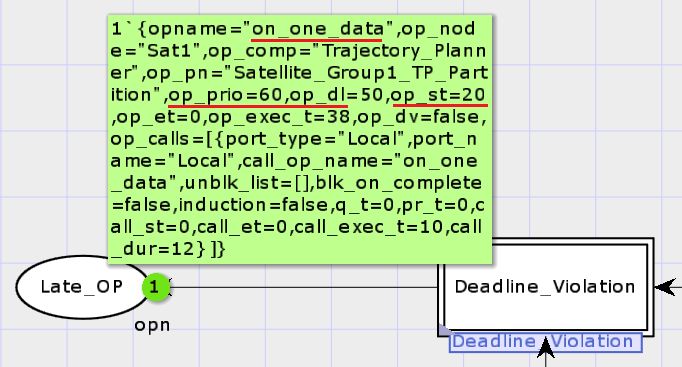
\includegraphics[width=0.29\textwidth]{cpn_tpa_dv_marking}
\caption{Observed Deadline Violation}
\label{fig:cpn_tpa_dv_marking}
\vspace{-0.2in}
\end{figure}
\vspace{0.1in}

\begin{figure}[ht]
\centering
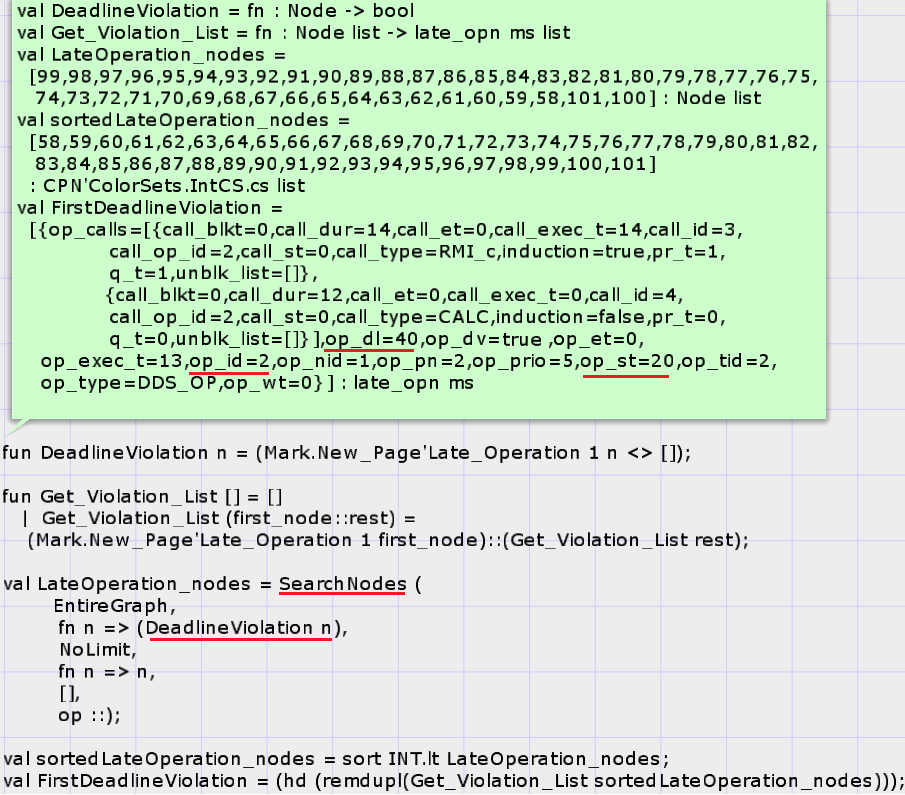
\includegraphics[width=0.5\textwidth]{cpn_tpa_dv_ss}
\caption{State Space Query for Deadline Violation Detection}
\label{fig:cpn_tpa_dv_ss}
\vspace{-0.2in}
\end{figure}
%\vspace{0.1in}

\subsection{Worst-case Trigger-to-Response Time Calculation}

As component operations run to completion, the analysis model keeps track of operation completion using a \emph{Completed\_Operations} place as shown in Figure \ref{fig:cpn_completed_operations}. 

\begin{figure}[ht]
\centering
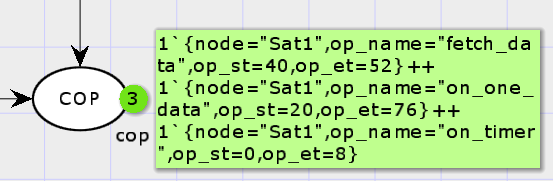
\includegraphics[width=0.35\textwidth]{cpn_completed_operations}
\caption{Completed Operations}
\label{fig:cpn_completed_operations}
\vspace{-0.2in}
\end{figure}
\vspace{0.1in}

For a known trigger operation and desired response operation, the worst-case trigger-to-response time can also be calculated from the generated state space. This is especially useful when multiple threads of same priority share a partition leading to a tree of possible thread execution orders. Once the necessary partial state space is generated, by using the operation IDs of the trigger and response, the earliest completion of the trigger operation and the latest completion of the response operation within the set period are identified. In the Trajectory Planning application, considering the \emph{TIMER\_OP} (\emph{op\_id = 1}) to be the trigger and the trajectory planning \emph{DDS\_OP} to be the response, the worst-case response time is found to be 65 ms as shown in Figure \ref{fig:cpn_tpa_trigger_response_time}. Since all of the necessary information is already packed in the state space, variants of such queries can be easily constructed without changing the model.

\begin{figure}[ht]
\centering
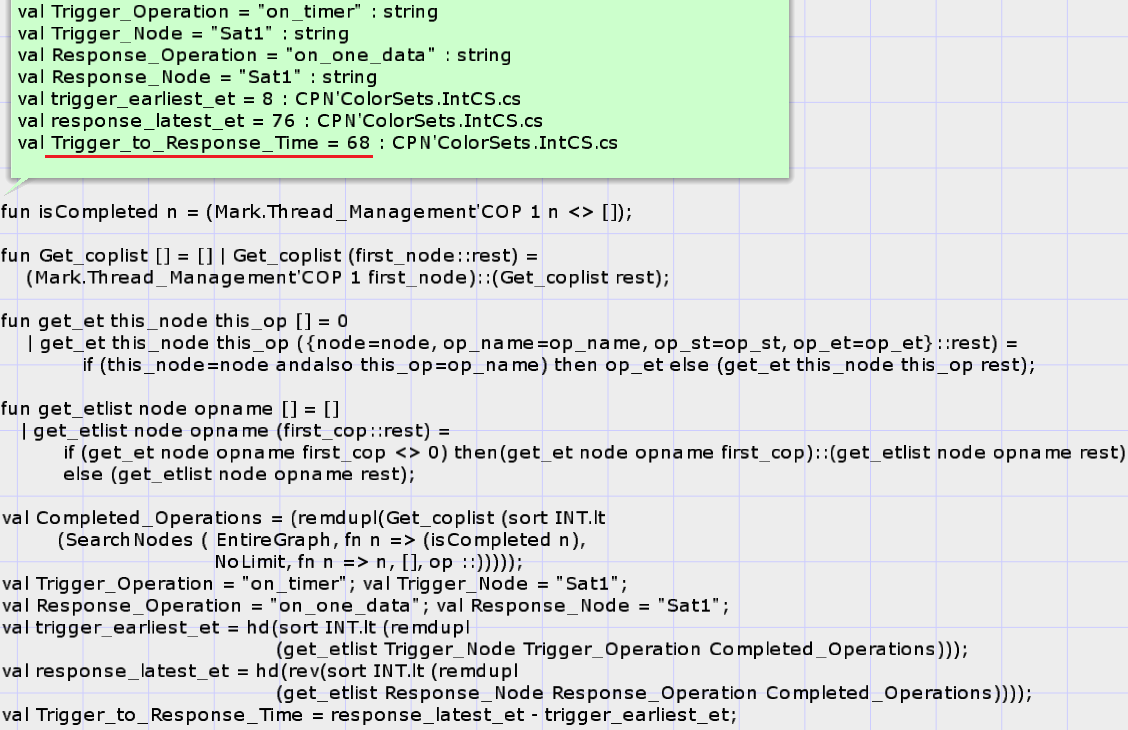
\includegraphics[width=0.5\textwidth]{cpn_tpa_trigger_response_time}
\caption{Worst-Case Trigger-to-Response Time Calculation}
\label{fig:cpn_tpa_trigger_response_time}
\vspace{-0.2in}
\end{figure}
\vspace{0.1in}

\subsection{Partial Thread Execution Order Generation}

Since the start and end time stamps of any completed operation can be obtained from the state space, this feature can be exploited to obtain a partial thread execution order and therefore thread priorities for applications in the design process. Consider the sample application shown in Figure \ref{fig:partial_order_example}.

\vspace{-0.08in}
\begin{figure}[ht]
\centering
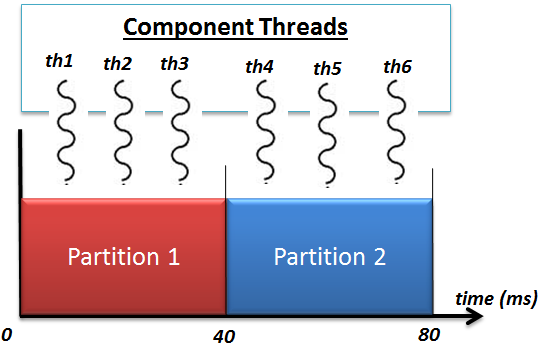
\includegraphics[width=0.25\textwidth]{partial_order_example}
\caption{Sample Application in Design Process}
\label{fig:partial_order_example}
\vspace{-0.16in}
\end{figure}

This application consists of 6 component executor threads that service component operation requests. Threads 1, 2, and 3 are assigned to Partition 1 and threads 4, 5, and 6 are assigned to Partition 2. The thread priorities and execution orders are unknown. Each component is associated with a timer that triggers an operation once every major frame, taking up to 8 ms to complete. The design requires that operation 3 (handled by thread 3) must complete before 20 ms and operation 5 (handled by thread 5) must complete before 60 ms from start of schedule. Figure \ref{fig:cpn_partial_order} shows queries that use the generated state space to obtain a thread execution order that satisfies such timing constraints. All threads are assigned the same priority and scheduling is therefore Round-Robin. The generated state space (size = 5000 nodes) records all possible thread execution orders for one hyperperiod of the schedule. From this partial state space, the state space node that first satisfies the timing requirement is identified. By generating a backtrace from the initial node and identifying the subset of nodes where the system clock ticks, the thread execution order is determined. It is clear that as the timing requirements become stricter, the number of possible thread execution orders decrease. For multiple timing requirements, if the set of thread execution orders contradict each other, the order that satisfies the higher priority timing requirement is chosen.

\vspace{-0.08in}
\begin{figure}[ht] 
\centering
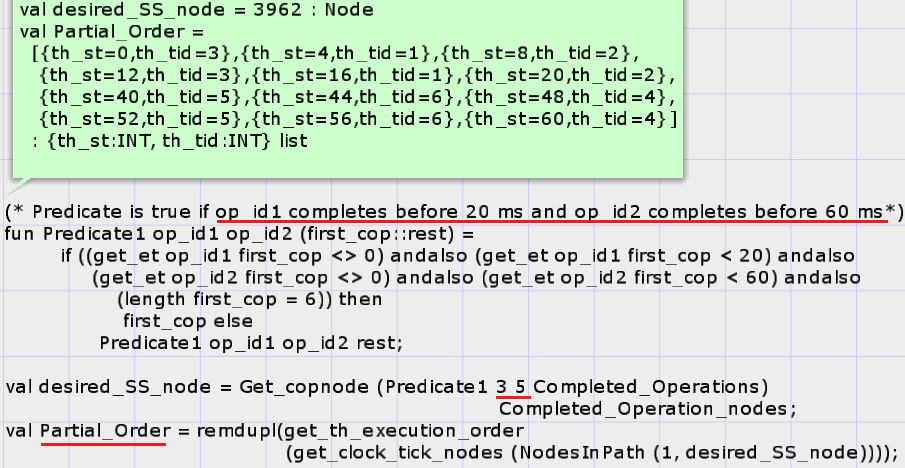
\includegraphics[width=0.5\textwidth]{cpn_partial_order}
\caption{Partial Order for Thread Execution}
\label{fig:cpn_partial_order}
\vspace{-0.18in}
\end{figure}

\subsection{Scalability Testing}
\label{subsec:Scalability_Testing}

The size of the generated state space is dependent on the amount of concurrency in the behavior. If all the executing threads had unique priorities, the thread execution order is a constant as the scheduling is priority-based. However, for larger systems with multiple applications and with threads of same priority sharing processor time in the same partition, several thread execution orders are possible depending on the arrival rates of operation requests and state of executing threads.  

Consider a set of mixed-criticality applications deployed on a 3-node satellite cluster. Each node has a unique temporal partition schedule with the longest schedule having a hyperperiod of 1 second, spanning 5 partitions. Hundred threads within the priority range [30-90] are distributed across the nodes. Most of the application component threads are triggered by timers of varying periodicity. In order to maximize the concurrency and possibilities of thread execution orders, most of the application threads are assigned the same priority and are also completely independent of each other. Dependence between components forces certain thread execution behaviors and so this is avoided. The Analysis model has 14 transitions and 11 places of which 3 places are observer places. Structural reductions to the model further reduce the state space size. Table \ref{tbl:scalability} summarizes the results of this effort. One of the observed consequences for such large systems is that the CPN Tools user interface suffers a rendering lag when it has to keep track of and display large token sets. This can be avoided by hiding as much detail as possible using hierarchy. 

\begin{table}[htbp]
\centering
\caption{Scalability Testing}
\begin{tabular}{| c | c | c | c | p{1.3cm} |}
\hline
 Satellites & Threads & Hyperperiods & State Space Nodes \\\hline
%TPA & 1 & 2 & 10 & 1500 \\\hline
%TPA & 2 & 2 & 10 & 3500 \\\hline
%TPA & 3 & 2 & 10 & 15000 \\\hline
%TPA & 4 & 2 & 10 & 30000 \\\hline
%TPA & 5 & 2 & 10 & 90000 \\\hline
1 & 50 & 10 & 125,000 \\\hline
3 & 100 & 10 & 480,000 \\\hline
\end{tabular}
\label{tbl:scalability}
\end{table}
\vspace{-0.1in}

\section{Analysis Model Generation}
\label{sec:Model_Generation}

For large applications, with several timers and component interaction patterns, hand-writing the CPN token specification will prove to be cumbersome and error prone. This can be avoided by integrating the temporal behavior specification for component-based applications onto the modeling framework used to generate the deployment plans and infrastructure glue code, effectively closing the loop shown in Figure \ref{fig:big_picture}. Since the structure of the places, transitions, color-sets, variables and function declarations do not change, only the application-specific token structure needs to be derived from the design model of the application. Figure \ref{fig:model_generation} shows a part of the ANTLR-based \cite{ANTLR_BOOK} specification grammar, a part of the input text file and the generated CPN tokens. 

\begin{figure}[ht] 
\centering
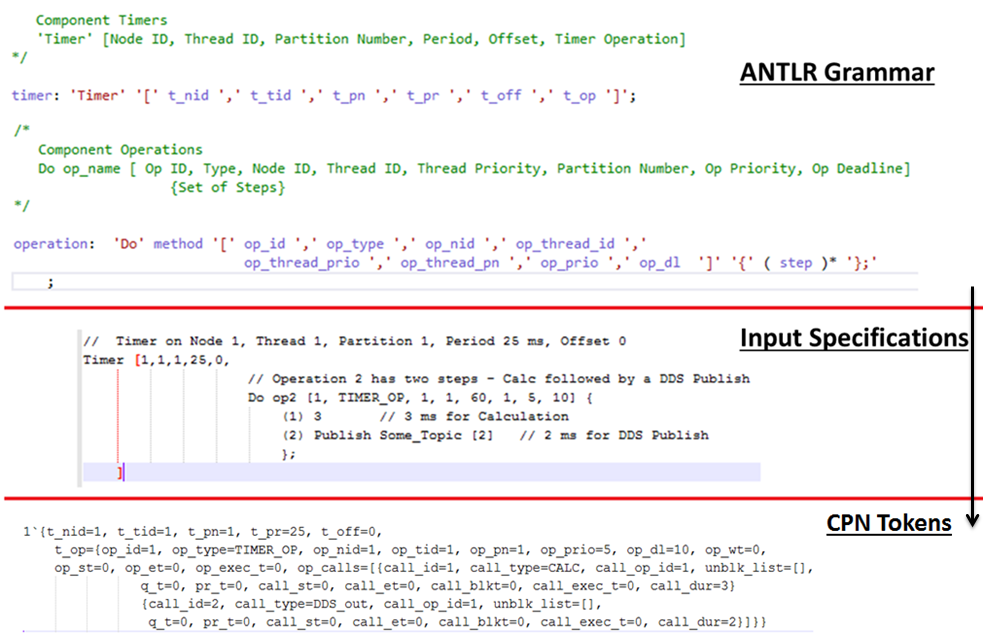
\includegraphics[width=0.5\textwidth]{model_generation}
\caption{Analysis Model Generation}
\label{fig:model_generation}
\vspace{-0.2in}
\end{figure}

\section{Discussion}
\label{sec:Discussion}

One of the main concerns in comprehensive design-time analysis of this kind is scalability. As the determinism in the initial design increases, the number of possible behaviors and therefore the size of the state space decreases. In essence, the effort required for the analysis to be useful for a designer is dependent heavily on the initial design itself. With increasing number of timer operations and equal priority threads sharing a CPU, the number of possible thread execution orders and behavioral scenarios will exponentially grow, leading to unmanageable state space sizes. The results shown in Table \ref{tbl:scalability} do not represent an upper bound on the state space size but one corresponding to an average-case scenario. For safety-critical systems, deterministic system behavior requires deterministic system designs. Since worst-case estimates are considered, it is unlikely that the actual system behavior would even reach certain behavioral regions. Therefore, the analysis results obtained from this approach effectively behave as guidelines for a more refined, and predictable application design as opposed to hard constraints on possible design.  
